\section{Cascata}

\begin{frame}
\begin{block}{Como desenvolver software/Games?}
	 \begin{itemize}
			  \item Podemos sair codificando.... até atingir um objetivo (Code and fix). Basicamente como fazemos 								exercícios programa da faculdade? Funciona? Há algum problema nessa abordagem?
			  \item Podemos usar alguma metodologia para garantir alguma qualidade nas diversas etapas da construção de um software/game
			  \item Uma metodologia clássica é a: metodologia cascata...
	 \end{itemize}
\end{block}
\end{frame}

\begin{frame}
\begin{block}{}
	 \begin{figure}[!htb]
			\centering	  				
			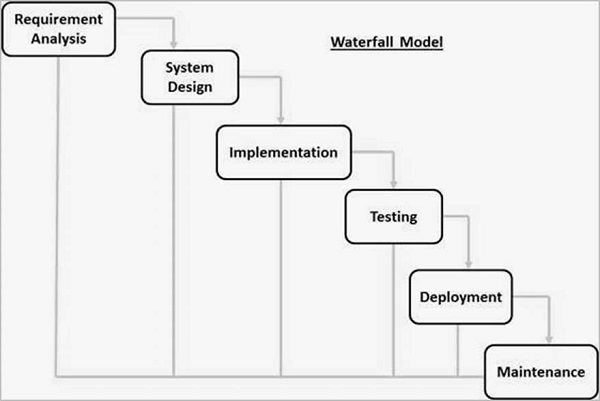
\includegraphics[height=7cm, width = 11cm]{./pic/sdlc_waterfall_model.jpg}
			\caption{Etapas da metodologia cascata}
			\label{fig_cascata}
		\end{figure}
\end{block}
\end{frame}


\begin{frame}
\begin{block}{Detalhes}
	 \begin{itemize}
			 \item As etapas são bem determinadas, tem começo meio e fim bem definidos e assume os requisitos são claros e bem definidos. Só passamos para a próxima etapa após finalizar com sucesso a etapa anterior. Não podem ocorrer alterações após as etapas

			 \item Começamos por especificar requisitos com o cliente, definir o que deve ser feito, como será feito.
			
			 \item O passo seguinte exige criar a arquitetura do sistema.
			
			 \item Após definir a arquitetura temos a codificação.
			
			 \item Testamos a codificação.
			
			 \item Entrega (Deploy).
			
			 \item Manutenção e correção de bugs.
	 \end{itemize}
\end{block}
\end{frame}

\begin{frame}
\begin{block}{Trade-off}
	 \begin{itemize}
			\item É simples e de fácil gerenciamento, afinal todas as etapas são rígidas e não permitem alterações.

			\item É bom para projetos pequenos onde os requisitos são extremamente bem definidos, conhecidos, não mudam e que precisam de uma extensa documentação.
			
			\item No mundo real ninguém conhece 100\% todos os requisitos no começo do projeto.... Nem mesmo o cliente ou usuário... Muito menos o desenvolvedor...
			
			\item Se ocorrer alguma alteração nessa metodologia ocorrerá um caos no projeto...
			
			\item Software só é entregue para o cliente/usuário depois que tudo está pronto.

	 \end{itemize}
\end{block}
\end{frame}

\begin{frame}
\begin{block}{Exercício}
	 \begin{itemize}
			\item Vamos simular desenvolver um projeto usando a metodologia: “cascata”.

			\item O jogo que iremos desenvolver será: ''Age of Empires", todos conhecem?
			
			\item Vamos escrever no papel, de forma sequencial cada etapa, somente começaremos outra etapa quando acabar a anterior. Devemos descrever/desenhar cada uma das etapas (Sejam criativos) 
			
			\item Requisitos (O professor fará o papel do cliente)
			
			\item Desenho da arquitetura do sistema (O professor fará o papel do gerente)
			
			\item Implementação
			
			\item Teste

			\item Deploy
			
			\item Manutenção

	 \end{itemize}
\end{block}
\end{frame}
